%% abtex2-modelo-trabalho-academico.tex, v-1.9.2 laurocesar
%% Copyright 2012-2014 by abnTeX2 group at http://abntex2.googlecode.com/ 
%%
%% This work may be distributed and/or modified under the
%% conditions of the LaTeX Project Public License, either version 1.3
%% of this license or (at your option) any later version.
%% The latest version of this license is in
%%   http://www.latex-project.org/lppl.txt
%% and version 1.3 or later is part of all distributions of LaTeX
%% version 2005/12/01 or later.
%%
%% This work has the LPPL maintenance status ``'maintained'.
%% 
%% The Current Maintainer of this work is the abnTeX2 team, led
%% by Lauro César Araujo. Further information are available on 
%% http://abntex2.googlecode.com/
%%
%% This work consists of the files abntex2-modelo-trabalho-academico.tex,
%% abntex2-modelo-include-comandos and abntex2-modelo-references.bib
%%

% ------------------------------------------------------------------------
% ------------------------------------------------------------------------
% abnTeX2: Modelo de Trabalho Academico (tese de doutorado, dissertacao de
% mestrado e trabalhos monograficos em geral) em conformidade com 
% ABNT NBR 14724:2011: Informacao e documentacao - Trabalhos academicos -
% Apresentacao
% ------------------------------------------------------------------------
% ------------------------------------------------------------------------

\documentclass[
	% -- opções da classe memoir --
	12pt,				% tamanho da fonte
	openright,			% capítulos começam em pág ímpar (insere página vazia caso preciso)
	twoside,			% para impressão em verso e anverso. Oposto a oneside
	a4paper,			% tamanho do papel. 
	% -- opções da classe abntex2 --
	%chapter=TITLE,		% títulos de capítulos convertidos em letras maiúsculas
	%section=TITLE,		% títulos de seções convertidos em letras maiúsculas
	%subsection=TITLE,	% títulos de subseções convertidos em letras maiúsculas
	%subsubsection=TITLE,% títulos de subsubseções convertidos em letras maiúsculas
	% -- opções do pacote babel --
	english,			% idioma adicional para hifenização
	% french,				% idioma adicional para hifenização
	% spanish,			% idioma adicional para hifenização
	brazil				% o último idioma é o principal do documento
	]{abntex2}

% ---
% Pacotes básicos 
% ---
\usepackage{lmodern}			% Usa a fonte Latin Modern			
\usepackage[T1]{fontenc}		% Selecao de codigos de fonte.
\usepackage[utf8]{inputenc}		% Codificacao do documento (conversão automática dos acentos)
\usepackage{lastpage}			% Usado pela Ficha catalográfica
\usepackage{indentfirst}		% Indenta o primeiro parágrafo de cada seção.
\usepackage{color}				% Controle das cores
\usepackage{graphicx}			% Inclusão de gráficos
\usepackage{microtype} 			% para melhorias de justificação
% ---
		
% ---
% Pacotes adicionais, usados apenas no âmbito do Modelo Canônico do abnteX2
% ---
\usepackage{lipsum}				% para geração de dummy text
% ---

% ---
% Pacotes de citações
% ---
\usepackage[brazilian,hyperpageref]{backref}	 % Paginas com as citações na bibl
\usepackage[alf]{abntex2cite}	% Citações padrão ABNT

% ---
% Pacotes adicionados por Rodrigo Cichetto
% ---
\usepackage{breakurl}
\usepackage{hyperref}
% CODES JS
\usepackage{listings}
\usepackage{color}
\definecolor{lightgray}{rgb}{.95,.95,.95}
\definecolor{darkgray}{rgb}{.4,.4,.4}
\definecolor{purple}{rgb}{0.65, 0.12, 0.82}

% ---
% CONFIGURAÇÃO RODRIGO
% ---
% CODES JS
\lstdefinelanguage{JavaScript}{
  keywords={typeof, new, true, false, catch, function, return, null, catch, switch, var, if, in, while, do, else, case, break},
  keywordstyle=\color{blue}\bfseries,
  ndkeywords={class, export, boolean, throw, implements, import, this},
  ndkeywordstyle=\color{darkgray}\bfseries,
  identifierstyle=\color{black},
  sensitive=false,
  comment=[l]{//},
  morecomment=[s]{/*}{*/},
  commentstyle=\color{purple}\ttfamily,
  stringstyle=\color{red}\ttfamily,
  morestring=[b]',
  morestring=[b]"
}

\lstset{
   language=JavaScript,
   backgroundcolor=\color{lightgray},
   extendedchars=true,
   basicstyle=\footnotesize\ttfamily,
   showstringspaces=false,
   showspaces=false,
   numbers=left,
   numberstyle=\footnotesize,
   numbersep=9pt,
   tabsize=4,
   breaklines=true,
   showtabs=false,
   captionpos=b
}


% --- 
% CONFIGURAÇÃO DE FIGURAS
% --- 
\graphicspath{ {imagens/} }

% --- 
% CONFIGURAÇÕES DE PACOTES
% --- 

% ---
% Configurações do pacote backref
% Usado sem a opção hyperpageref de backref
\renewcommand{\backrefpagesname}{Citado na(s) página(s):~}
% Texto padrão antes do número das páginas
\renewcommand{\backref}{}
% Define os textos da citação
\renewcommand*{\backrefalt}[4]{
	\ifcase #1 %
		Nenhuma citação no texto.%
	\or
		Citado na página #2.%
	\else
		Citado #1 vezes nas páginas #2.%
	\fi}%
% ---

% ---
% Informações de dados para CAPA e FOLHA DE ROSTO
% ---
\titulo{Desenvolvimento de aplicações com JavaScript }
\autor{Rodrigo Cichetto Monteiro}
\local{Brasil}
\data{2018}
\orientador{Leandro Carlos Fernandes}
% \coorientador{Danielle Colturato}
\instituicao{%
  Universidade Paulista -- UNIP
  \par
  Faculdade de Ciência da Computação
  \par
  Programa de Graduação}
\tipotrabalho{Tese (Graduação)}
% O preambulo deve conter o tipo do trabalho, o objetivo, 
% o nome da instituição e a área de concentração 
\preambulo{Trabalho apresentado a UNIP - UNIVERSIDADE PAULISTA
como pré-requisito
para obtenção da Certificação de Conclusão do
Curso de Bacharelado em Ciência da Computação.
Orientador: Prof. \imprimirorientador}
% ---


% ---
% Configurações de aparência do PDF final

% alterando o aspecto da cor azul
\definecolor{blue}{RGB}{41,5,195}

% informações do PDF
\makeatletter
\hypersetup{
     	%pagebackref=true,
		pdftitle={\@title}, 
		pdfauthor={\@author},
    	pdfsubject={\imprimirpreambulo},
	    pdfcreator={LaTeX with abnTeX2},
		pdfkeywords={abnt}{latex}{abntex}{abntex2}{trabalho acadêmico}, 
		colorlinks=true,       		% false: boxed links; true: colored links
    	linkcolor=blue,          	% color of internal links
    	citecolor=blue,        		% color of links to bibliography
    	filecolor=magenta,      		% color of file links
		urlcolor=blue,
		bookmarksdepth=4
}
\makeatother
% --- 

% --- 
% Espaçamentos entre linhas e parágrafos 
% --- 

% O tamanho do parágrafo é dado por:
\setlength{\parindent}{1.3cm}

% Controle do espaçamento entre um parágrafo e outro:
\setlength{\parskip}{0.2cm}  % tente também \onelineskip

% ---
% compila o indice
% ---
\makeindex
% ---

% ----
% Início do documento
% ----
\begin{document}

% Retira espaço extra obsoleto entre as frases.
\frenchspacing 

% ----------------------------------------------------------
% ELEMENTOS PRÉ-TEXTUAIS
% ----------------------------------------------------------
% \pretextual

% ---
% Capa
% ---
\imprimircapa
% ---

% ---
% Folha de rosto
% (o * indica que haverá a ficha bibliográfica)
% ---
\imprimirfolhaderosto*
% ---

% ---
% Inserir a ficha bibliografica
% ---

% Isto é um exemplo de Ficha Catalográfica, ou ``Dados internacionais de
% catalogação-na-publicação''. Você pode utilizar este modelo como referência. 
% Porém, provavelmente a biblioteca da sua universidade lhe fornecerá um PDF
% com a ficha catalográfica definitiva após a defesa do trabalho. Quando estiver
% com o documento, salve-o como PDF no diretório do seu projeto e substitua todo
% o conteúdo de implementação deste arquivo pelo comando abaixo:
%
% \begin{fichacatalografica}
%     \includepdf{fig_ficha_catalografica.pdf}
% \end{fichacatalografica}
\begin{fichacatalografica}
	\vspace*{\fill}					% Posição vertical
	\hrule							% Linha horizontal
	\begin{center}					% Minipage Centralizado
	\begin{minipage}[c]{12.5cm}		% Largura
	
	\imprimirautor
	
	\hspace{0.5cm} \imprimirtitulo  / \imprimirautor. --
	\imprimirlocal, \imprimirdata-
	
	\hspace{0.5cm} \pageref{LastPage} p. : il. (algumas color.) ; 30 cm.\\
	
	\hspace{0.5cm} \imprimirorientadorRotulo~\imprimirorientador\\
	
	\hspace{0.5cm}
	\parbox[t]{\textwidth}{\imprimirtipotrabalho~--~\imprimirinstituicao,
	\imprimirdata.}\\
	
	\hspace{0.5cm}
		1. JavaScript.
        2. Arquitetura multicamadas.
        3. MEAN Stack.
		I. Orientador \imprimirorientador.
		II. Universidade Paulista -- UNIP.
		III. Faculdade de Ciência da Computação.
		IV. \imprimirtitulo 
		V. \imprimirautor
	
	\hspace{8.75cm} CDU 02:141:005.7\\
	
	\end{minipage}
	\end{center}
	\hrule
\end{fichacatalografica}
% ---

% ---
% Inserir errata
% ---
% \begin{errata}
% Elemento opcional da \citeonline[4.2.1.2]{NBR14724:2011}. Exemplo:

% \vspace{\onelineskip}

% FERRIGNO, C. R. A. \textbf{Tratamento de neoplasias ósseas apendiculares com
% reimplantação de enxerto ósseo autólogo autoclavado associado ao plasma
% rico em plaquetas}: estudo crítico na cirurgia de preservação de membro em
% cães. 2011. 128 f. Tese (Livre-Docência) - Faculdade de Medicina Veterinária e
% Zootecnia, Universidade de São Paulo, São Paulo, 2011.

% \begin{table}[htb]
% \center
% \footnotesize
% \begin{tabular}{|p{1.4cm}|p{1cm}|p{3cm}|p{3cm}|}
%   \hline
%    \textbf{Folha} & \textbf{Linha}  & \textbf{Onde se lê}  & \textbf{Leia-se}  \\
%     \hline
%     1 & 10 & auto-conclavo & autoconclavo\\
%    \hline
% \end{tabular}
% \end{table}
% \end{errata}
% ---

% ---
% Inserir folha de aprovação
% ---

% Isto é um exemplo de Folha de aprovação, elemento obrigatório da NBR
% 14724/2011 (seção 4.2.1.3). Você pode utilizar este modelo até a aprovação
% do trabalho. Após isso, substitua todo o conteúdo deste arquivo por uma
% imagem da página assinada pela banca com o comando abaixo:
%
% \includepdf{folhadeaprovacao_final.pdf}
%
\begin{folhadeaprovacao}

  \begin{center}
    {\ABNTEXchapterfont\large\imprimirautor}

    \vspace*{\fill}\vspace*{\fill}
    \begin{center}
      \ABNTEXchapterfont\bfseries\Large\imprimirtitulo
    \end{center}
    \vspace*{\fill}
    
    \hspace{.45\textwidth}
    \begin{minipage}{.5\textwidth}
        \imprimirpreambulo
    \end{minipage}%
    \vspace*{\fill}
   \end{center}
        
   Trabalho aprovado. \imprimirlocal, 24 de novembro de 2018:

   \assinatura{\textbf{\imprimirorientador} \\ Orientador} 
   \assinatura{\textbf{Professor} \\ Convidado 1}
   \assinatura{\textbf{Professor} \\ Convidado 2}
   %\assinatura{\textbf{Professor} \\ Convidado 3}
   %\assinatura{\textbf{Professor} \\ Convidado 4}
      
   \begin{center}
    \vspace*{0.5cm}
    {\large\imprimirlocal}
    \par
    {\large\imprimirdata}
    \vspace*{1cm}
  \end{center}
  
\end{folhadeaprovacao}
% ---

% ---
% Dedicatória
% ---
\begin{dedicatoria}
    \vspace*{\fill}
    \centering
    \noindent
    \textit{ Este trabalho é dedicado aos meus pais,\\
    pelo apoio em todos os momentos.} \vspace*{\fill}
 \end{dedicatoria}
% \begin{dedicatoria}
%    \vspace*{\fill}
%    \centering
%    \noindent
%    \textit{ Este trabalho é dedicado às crianças adultas que,\\
%    quando pequenas, sonharam em se tornar cientistas.} \vspace*{\fill}
% \end{dedicatoria}
% ---

% ---
% Agradecimentos
% ---
% \begin{agradecimentos}
% Os agradecimentos principais são direcionados à Gerald Weber, Miguel Frasson,
% Leslie H. Watter, Bruno Parente Lima, Flávio de Vasconcellos Corrêa, Otavio Real
% Salvador, Renato Machnievscz\footnote{Os nomes dos integrantes do primeiro
% projeto abn\TeX\ foram extraídos de
% \url{http://codigolivre.org.br/projects/abntex/}} e todos aqueles que
% contribuíram para que a produção de trabalhos acadêmicos conforme
% as normas ABNT com \LaTeX\ fosse possível.
% Agradecimentos especiais são direcionados ao Centro de Pesquisa em Arquitetura
% da Informação\footnote{\url{http://www.cpai.unb.br/}} da Universidade de
% Brasília (CPAI), ao grupo de usuários
% \emph{latex-br}\footnote{\url{http://groups.google.com/group/latex-br}} e aos
% novos voluntários do grupo
% \emph{\abnTeX}\footnote{\url{http://groups.google.com/group/abntex2} e
% \url{http://abntex2.googlecode.com/}}~que contribuíram e que ainda
% contribuirão para a evolução do \abnTeX.
% \end{agradecimentos}
% ---

% ---
% Epígrafe
% ---
\begin{epigrafe}
    \vspace*{\fill}
	\begin{flushright}
		\textit{``Ser o homem mais rico do cemitério não me interessa.\\
		Ir para a cama à noite dizendo que fizemos algo maravilhoso, \\ isso importa para mim. \\
		(Steve Jobs; The Wall Street Journal, 1993.)}
	\end{flushright}
\end{epigrafe}
% ---

% ---
% RESUMOS
% ---

% resumo em português
\setlength{\absparsep}{18pt} % ajusta o espaçamento dos parágrafos do resumo
\begin{resumo}
%  Segundo a \citeonline[3.1-3.2]{NBR6028:2003}
Já pensou em criar uma rápida prototipação de software ou desenvolver aplicações escaláveis de forma rápida e utilizando apenas uma linguagem? Isso é possível e traz benefícios a empresa, desenvolvedores e até mesmo ao cliente. Nos últimos tempos o JavaScript ganhou muita importância em quaisquer cenários, e vem sendo utilizada em sites, aplicações, \textit{mobile}, servidores, automação de testes, automação de tarefas, internet das coisas, entre outros. Este trabalho tem como principal objetivo apresentar benefícios de utilizar a linguagem JavaScript em todas as camadas do desenvolvimento, destacando ferramentas já existentes aplicadas à arquitetura multicamadas. Mas lembre-se com grandes poderes vem grandes responsabilidades.

 \vspace{\onelineskip}

 \textbf{Palavras-chaves}: javascript, arquitetura multicamadas, frameworks
\end{resumo}

% resumo em inglês
\begin{resumo}[Abstract]
 \begin{otherlanguage*}{english}

Have you thought about creating a rapid prototyping of software or developing scalable applications quickly and using only one programming language? This is possible and brings benefits to the company, developers and even the customer. In recent times JavaScript has gained a lot of importance in any scenario, and has been used in websites, applications, mobile, servers, automation of tests, automation of tasks, internet of things, among others. This work has as main objective to present benefits of using the JavaScript language in all layers of development, highlighting existing tools applied to multilayer architecture. But remember with great powers comes great responsibilities.

   \vspace{\onelineskip}
 
   \noindent 
   \textbf{Key-words}: javascript, multilayer architecture, frameworks
 \end{otherlanguage*}
\end{resumo}
% ---
% inserir lista de ilustrações
% ---
\pdfbookmark[0]{\listfigurename}{lof}
\listoffigures*
\cleardoublepage
% ---

% ---
% inserir lista de tabelas
% ---
% \pdfbookmark[0]{\listtablename}{lot}
% \listoftables*
% \cleardoublepage
% ---

% ---
% inserir lista de abreviaturas e siglas
% ---
\begin{siglas}
%   \item[ABNT] Associação Brasileira de Normas Técnicas
%   \item[abnTeX] ABsurdas Normas para TeX
  \item[JS] JavaScript
  \item[HTML] Abreviação para \textit{HyperText Markup Language}, que em português significa Linguagem de Marcação de Hipertexto.
  \item[DOM] Abreviação para \textit{Document Object Model}, que em português significa Modelo de Objetos e Documentos.
  \item[CSS] Abreviação para \textit{Cascading Style Sheets}, que em português significa Folhas de Estilo em Cascata.
  \item[ECMA] Abreviação para \textit{European Computer Manufacturers Association}, que em português significa Associação Européia de Fabricantes de Computadores.
  \item[API] Abreviação para \textit{Application Programming Interface}, que em português significa Interface de programação de aplicações.
  \item[REST] Abreviação para \textit{Representational State Transfer}, que em português significa Transferência de Estado Representacional.
  \item[HTTP] Abreviação para \textit{Hypertext Transfer Protocol}, que em português significa Protocolo de Transferência de Hipertexto.
  \item[URI] Abreviação para \textit{Uniform Resource Identifier}, que em português significa Identificador Uniforme de Recurso.
  \item[SQL] Abreviação para \textit{Structured Query Language}, que em português significa Linguagem de Consulta Estruturada.
\end{siglas}
% ---

% ---
% inserir lista de símbolos
% ---
% \begin{simbolos}
% 	\item
% %   \item[$ \in $] Pertence
% \end{simbolos}
% ---

% ---
% inserir o sumariopr
% ---
\pdfbookmark[0]{\contentsname}{toc}
\tableofcontents*
\cleardoublepage
% ---

% TODO inserir SOBRE O AUTOR

% ----------------------------------------------------------
% ELEMENTOS TEXTUAIS
% ----------------------------------------------------------
\textual

% ----------------------------------------------------------
% Introdução (exemplo de capítulo sem numeração, mas presente no Sumário)
% ----------------------------------------------------------
% \chapter*[Introdução]{Introdução}
% \addcontentsline{toc}{chapter}{Introdução}

% -----------------------------------
% CHAPTER:
% Introdução
% -----------------------------------
\chapter{Introdução}

Inicialmente implementada com o objetivo no desenvolvimento web para o lado do cliente, a linguagem criada por Brendan Eich enquanto trabalhou na Netscape, tornou-se uma das linguagens mais populares da atualidade. 

Nos últimos anos a linguagem JavaScript ganhou maior importância, com o surgimento de bibliotecas e \textit{frameworks} que possibilitaram o desenvolvimento de não somente web sites mas também aplicativos, \textit{single page applications}, programas \textit{desktop}, \textit{progressive web apps} e muito mais.

O surgimento do Node.js trouxe novas possibilidades para os desenvolvedores, levando a linguagem para um novo patamar. Criado com um modelo não bloqueante na entrada e saída de dados, possibilitou que a linguagem fosse levada agora também para aplicações \textit{back-end}, ou seja, para o \textit{server-side} (lado do servidor). % *

Trabalhar com JavaScript em diversas plataformas como \textit{client-side} e \textit{server-side} a tempos atras poderia ser considerado uma utopia. Graças ao crescimento da linguagem agora é possivel a execução da linguagem nos mais diversos ambientes. %*

% ---
% Objetivos
% ---
\section{Objetivos}

O trabalho tem como objetivo relatar a evolução da linguagem JavaScript e sua ampla utilização, para os mais diferentes tipos de sistemas, no contexto atual.

Não há soluções tecnológicas a serem resolvidas neste projeto, nele é apresentado informações e tecnologias já existentes, que se encaixem com a arquitetura apresentada e que compartilhem da mesma linguagem.

% -----------------------------------
% CHAPTER:
% Pesquisa bibliográfica
% -----------------------------------
\chapter{Revisão bibliográfica}

% ---
% Uma linguagem em todo o desenvolvimento
% ---
\section{Uma linguagem para todo o desenvolvimento}
\label{sec:UmaLinguagemDesenvolvimento}

Por que não em vez de utilizar uma linguagem para o \textit{client-side} e outra para o \textit{server-side}, utilizar apenas uma linguagem para ambos? Ao utilizar a mesma linguagem em todas as camadas de uma aplicação, você traz vantagens para o projeto, equipe e até mesmo para o cliente final. Todo mundo ganha!

A vantagem mais clara que temos é a padronização, o ser humano tem uma enorme facilidade no reconhecimento de padrões, por tudo ser escrito na mesma linguagem a uniformidade é maior, tornando assim o trabalho mais compreensivo para os programadores envolvidos no projeto, seja ele \textit{front-end}, \textit{back-end} ou \textit{full-stack}. 

Se um programador compreende bem a linguagem ele será capaz também de desenvolver sobre todas as camadas, reduzindo o tempo ocioso de equipes que dependem do trabalho de outras equipes. Isso faz com que times \textit{front-end} e \textit{back-end} se tornem times \textit{full-stack} sendo assim mais versáteis, ágeis e que compreendem melhor o produto como um todo, trazendo assim benefícios também a empresa em suas contratações.

Outra vantagem a se considerar é a possibilidade de reaproveitar código. Reutilizar trechos de código é uma forma de reduzir a carga de trabalho dos desenvolvedores e acelerar o desenvolvimento. Além de objetos serem bem parecidos, se não idênticos, facilitando muito o debug e a comunicação entre aplicações e serviços.

Também há benefícios para o desenvolvedor, uma vez que conhecer uma linguagem que pode ser um elemento comum a vários \textit{frameworks} e de base para o desenvolvimento em qualquer ambiente.

Com todas essas vantagens atingimos também diretamente o cliente, que precisa esperar menos para seu projeto ficar pronto e consequentemente reduz o custo final do desenvolvimento.

A abordagem de se utilizar uma linguagem para todo o desenvolvimento, vem sendo muito utilizada em hackathons e competições curtas de programação, onde deve-se perder o menor tempo possível e com isso criar protótipos de forma rápida.

% ---
% JavaScript
% ---
\section{JavaScript}

As muitas vantagens de se utilizar o JavaScript fizeram com que ela se tornasse a linguagem de programação mais popular do mundo, desbancando até mesmo linguagens de maior expressão como Java, C\#, PHP, Phyton e outras.

JavaScript é uma linguagem de programação dinâmica interpretada, inicialmente utilizada pelos navegadores para execução de \textit{scripts} no lado do cliente, ou seja, no seu \textit{browser}. Os \textit{scripts} são incorporados a páginas HTML tendo como função adicionar interatividade para o usuário.

Atualmente, é impossível imaginar a internet sem a existência do JavaScript, certamente você já se deparou com alguns dos exemplos como os famosos carrosséis (Figura \ref{fig:JSExampleCarrousel}), as tão importantes validações de formulários (Figura \ref{fig:JSExampleValidation}), ou até mesmo com um \textit{modal} (Figura \ref{fig:JSExampleModal}) que mostram algumas das aplicações da linguagem em \textit{web sites}.

% \pagebreak
\begin{figure}[h]
	\centering

	\caption{\textit{Carrousel} - Um componente de apresentação de slides para percorrer imagens ou slides de texto - como um carrossel. -- Exemplo de aplicação do JS} \label{fig:JSExampleCarrousel}
    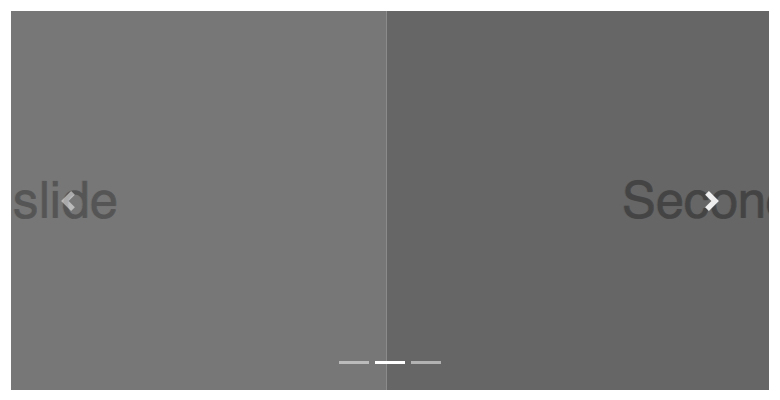
\includegraphics[scale=0.4]{js-example-carousel} \\
    Fonte: {Bootstrap \footnote{\url{https://getbootstrap.com/docs/4.1/components/carousel/}}}

    \caption{\textit{Validation} - Validação de formulários -- Exemplo de aplicação do JS} \label{fig:JSExampleValidation}
    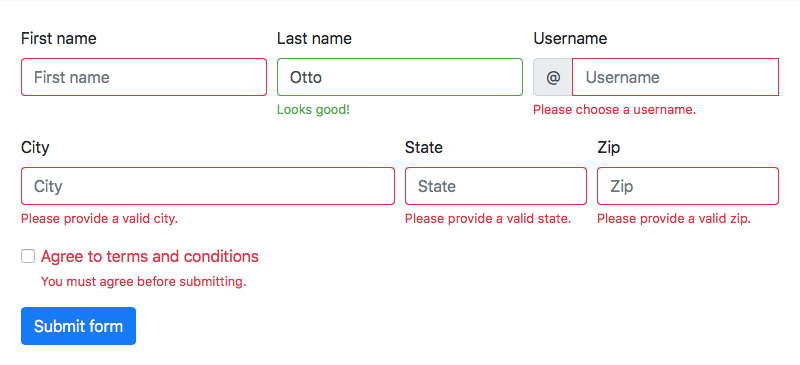
\includegraphics[scale=0.45]{js-example-validation} \\
    Fonte: {Bootstrap \footnote{\url{https://getbootstrap.com/docs/4.1/components/forms/}}}
	
    \caption{\textit{Modal} - Caixas de diálogo para notificações ao usuário. -- Exemplo de aplicação do JS} \label{fig:JSExampleModal}
    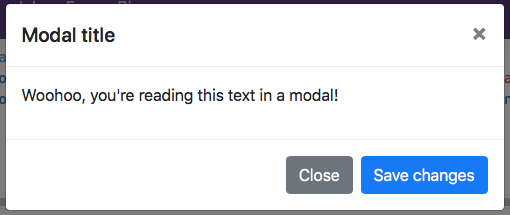
\includegraphics[scale=0.5]{js-example-modal} \\
    Fonte: {Bootstrap \footnote{\url{https://getbootstrap.com/docs/4.1/components/modal/}}}

\end{figure}

O JavaScript apresenta uma sintaxe simples que facilita o aprendizado, mas não confunda pois a primeira vista muitos desenvolvedores podem acreditar que a linguagem é defeituosa ou esquisita, pois não compreendem o real poder que se esconde por trás desta simplicidade. 

Inicialmente classificada como linguagem do tipo \textit{client side}, é por si só uma linguagem compacta, mas muito flexível, com comportamentos diferenciados das demais ela permite, por exemplo, que um objeto tenha seus atributos adicionados ou removidos em tempo de execução, o que não é muito comum para desenvolvedores de outras linguagens.

É uma linguagem interpretada, pois seus comandos são executados sem que haja necessidade de compilação, tendo como interpretador de \textit{script} o \textit{browser} do usuário. Sendo assim independente de plataformas, como os comandos são interpretados pelo navegador do usuário, é irrelevante se o usuário está utilizando Windows, Linux ou Mac OS.

Sua tipagem é dinâmica, ou seja, tipos são associados com valores. Por exemplo, uma variável pode ser associada a um número e posteriormente associada a um texto.

Com JavaScript também é possível a detecção de eventos, sempre que algo de importante acontece é disparado um evento, o clique de um botão, o preenchimento de um campo de formulário, a movimentação do mouse, são alguns exemplos dos eventos que são disparados. Isso nos permite reagir a estes eventos deixando assim que nossa aplicação deixe de ser estática.

Podemos executar códigos JS de várias formas na web, sendo uma delas pelo próprio console do navegador pressionando as teclas F12, importando um script em uma página HTML, ou até mesmo envolvendo o trecho de código na tag <script>.

No início da internet as páginas não eram nada interativas, documentos apresentavam seu conteúdo exatamente como foram criados para serem exibidos no navegador e só. O JavaScript revolucionou o que podemos fazer, hoje não só na web, mas praticamente em todas as áreas que se possa programar. 

\subsection{A linguagem nos dias atuais}

Se existe alguma linguagem que evoluiu nos últimos tempos, essa linguagem é o JavaScript. Conforme a linguagem evoluiu se tornou mais poderosa e independente do navegador. Isso possibilitou que a linguagem fosse utilizada não somente para a web como \textit{client side} mas agora em várias plataformas. 

\subsubsection{JavaScript além dos navegadores}
\label{subsec:JavaScriptAlemNavegadores}

Inicialmente tratada como um extra para os navegadores, podemos dizer que a linguagem caminhou com o avanço da tecnologia, isso possibilitou o uso da linguagem em diversas plataformas sendo algumas delas:

\begin{enumerate}[label=\alph*)]
\item Aplicações web
\item Aplicativos mobile 
\item Automação de testes e de tarefas
\item Controle de hardware
\item Desenvolvimento de jogos
\item Internet das coisas
\item Realidade virtual e aumentada
\item Softwares desktop
\item Servidores 
\end{enumerate}

Praticamente tudo que envolve programação o JavaScript está presente, para criar um software desktop existe por exemplo o \textit{framework} Electron \footnote{\url{https://electronjs.org}}, desenvolvido pelo GitHub ele possibilita criar aplicativos desktop multiplataforma através do JavaScript. No desenvolvimento de jogos a \textit{engine} Unity \footnote{\url{https://unity3d.com/pt}} é uma das plataformas que oferecem suporte a linguagem.

O ecossistema JavaScript é gigante e tem atraído empresas de todos os portes. Hoje grandes empresas como Google, Microsoft, Netflix, Uber e Linkedin usam JavaScript no \textit{back-end}. 

Isso acabou impactando o mundo dos desenvolvedores, fazendo com que seja obrigatório todo programador saber pelo menos o básico da linguagem, mesmo atuando em outras áreas, como \textit{back-end} e até mesmo teste de \textit{softwares}.

\subsubsection{ECMA}

Para a linguagem rodar em ambientes que podem variar, algo importante a considerar é a compatibilidade entre os navegadores. Para isso é necessário um padrão, tal criado e mantido até hoje pelo ECMA Internacional. 

Já em 1996 a Netscape, detentora do JavaScript, anunciou que submetia a linguagem para o ECMA Internacional como candidata a padrão industrial, resultando então no ECMAScript.

Padronização que define a estrutura da linguagem, seus comportamentos e comandos, dando assim um padrão aos interpretadores da linguagem. 

Como vimos, as vantagens do JavaScript vão muito além de ser a linguagem mais popular da web, ou de até mesmo possuir a maior comunidade de programadores. Depois de 2015, a partir do ES6 (ECMAScript 6) fez com que a linguagem passa-se por uma série de mudanças essenciais que fizeram com que a linguagem se consolidasse e desde então não parou de evoluir.

Atualmente a linguagem se encontra na 9ª edição chamada de ECMAScript 2018, finalizada em Junho de 2018.

Com participação colaborativa de empresas que implementam o \textit{run-time} da linguagem, como Mozilla, Google, Microsoft e Apple, além da participação de desenvolvedores da comunidade, o ECMA coordena e faz o trabalho de desenvolvimento contínuo e descentralizado do JS.

No site oficial\footnote{\url{http://www.ecma-international.org/publications/standards/Ecma-262.htm}} a ECMA disponibiliza informações como versão atual e a documentação da linguagem. Porém aconselho a buscar documentações na internet, uma boa referência a seguir é o site da Mozilla \footnote{\url{https://developer.mozilla.org/pt-BR/docs/Web/JavaScript}}, ou também o site da W3Schools \footnote{\url{https://www.w3schools.com/jsref/default.asp}}. 

A 10ª edição já está em desenvolvimento, devendo chegar até o final de Junho no ano de 2019, sendo chamada de ECMAScript 2019.

% ---
% Arquitetura
% ---
\section{Arquitetura}
\label{sec:Arquitetura}

% \citeauthor{sommerville_engenharia}
% \cite{sommerville_engenharia}

A arquitetura de um software consiste na definição de seus componentes, relacionamentos com softwares externos e suas propriedades. Na arquitetura multicamadas temos o famoso Cliente-Servidor onde as camadas de apresentação, processamento de aplicativos e gerenciamento de dados são separados.

Com este modelo de arquitetura isolamos funções da aplicação de forma modular, facilitando sua manutenção e depuração, além de criar uma hierarquia de níveis de acesso, protegendo as camadas mais internas.

Também conhecidas como stacks, as camadas de uma aplicação são basicamente o \textit{front-end} (cliente) e \textit{back-end} (servidor). Camadas são uma maneira de separar responsabilidades, uma camada superior pode usar serviços de uma camada inferior, mas não o oposto. 

A modularização refere-se a separar a lógica de negócios e regras de acesso ao banco de dados da camada de apresentação.

\begin{figure}[h]
	\centering

	\caption{Exemplo de arquitetura multicamadas} \label{fig:MultilayerArchitecture}
    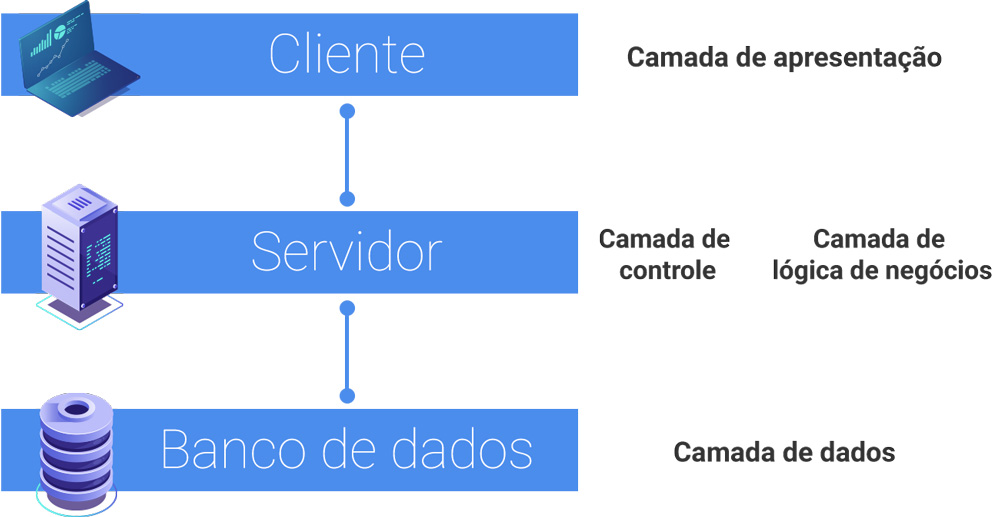
\includegraphics[scale=0.4]{multilayer-architecture}

\end{figure}

Na parte inferior da Figura \ref{fig:MultilayerArchitecture}, está localizado o servidor de banco de dados, no qual fornece os dados para os servidores da aplicação. Já na parte superior estão os clientes, que fazem a comunicação com a camada intermediária através da utilização de interfaces e protocolos de rede. Este é basicamente o esquema de comunicação desta arquitetura.

A arquitetura apresentada foi escolhida por criar um cenário de aplicação que exemplifica bem as separações das responsabilidades, podendo assim mostrar a aplicação de apenas uma linguagem em todos eles, assim como a flexibilidade do JavaScript.

\subsection{Cliente}
\label{subsec:Cliente}

O \textbf{Cliente} representa a \textbf{camada de apresentação}, ela é responsável pela interação com o usuário além de se comunicar com a camada de controle e ter o dever de garantir a consistência entre o dado e sua apresentação.

Para o cliente pouco importa as regras de negócio, uma vez que seu papel é enviar informações e espera receber os dados processados, além de ser responsável por executar lógica no lado do cliente. Aqui encontramos a parte da aplicação \textit{client-side}, em ambientes web também conhecida como \textit{front-end}.

Um benefício da modularização da arquitetura multicamadas nos possibilita é a criação de várias aplicações clientes que podem compartilhar as mesmas regras, pois ficam encapsuladas em uma camada de acesso comum. Por exemplo, posso ter um aplicativo e um web-site consumindo um mesmo serviço, compartilhando assim das mesmas regras.

Eliminando problemas que podem ocorrer no controle de versão em outros tipos de arquitetura, pois em uma arquitetura diferente da modular, se determinado usuário possui uma versão mais antiga do que outro, pode ocorrer erros de dados lógicos no processamento das regras de negócios, uma vez que não compartilham da mesma regra.

\subsection{Serviço}
\label{subsec:Servico}

O \textbf{Serviço} serve como \textbf{camada de controle}, onde recebe as requisições e comanda o fluxo servindo como uma camada intermediária entre a camada de apresentação e a lógica. De forma que o banco de dados e o servidor podem estar fisicamente distantes da aplicação cliente.

Normalmente a camada de controle costuma trabalhar junto da camada de lógica de negócios, ou seja o serviço trabalha junto com o servidor, resumidos a apenas uma camada.

Uma das formas de fazer essa comunicação é através de protocolos, como o \textit{HTTP} que através de um modelo, como por exemplo \textit{REST} nos permite realizar essa comunicação entre camadas.

\textit{REST} é um modelo descrito por Roy Fielding, um dos principais criadores do protocolo \textit{HTTP}, em sua tese de doutorado, que foi adotado como o modelo a ser utilizado na evolução da arquitetura do protocolo \textit{HTTP}, muitos desenvolvedores perceberam de que ele poderia também ser utilizado na implementação de \textit{Web Services}.

O modelo \textit{REST} utiliza como gerenciamento de informações os chamados recursos, que nada mais são do que uma abstração sobre um determinado tipo de informação que uma aplicação gerencia, sendo que um dos princípios é de que todo recurso deve possuir uma identificação única, também conhecidos como \textit{URI}.

\subsection{Servidor}
\label{subsec:Servidor}

Podemos considerar o \textbf{Servidor} como a \textbf{camada de lógicas de negócios}. Nela recebemos requisições devolvendo informações que podem ser processadas por esta própria camada ou retornar informações através da camada de acesso a dados. Aqui está a parte da aplicação \textit{server-side}, em ambientes web também conhecida como \textit{back-end}.

Modularizar a lógica de negócios também traz benefícios, por os clientes acessarem uma mesma camada em comum (servidor), qualquer alteração realizada nas regras de negócios serão vistas por todas as aplicações clientes.

Também nos possibilita escalabilidade, com a utilização de outras arquiteturas, é comum que ocorra uma queda de desempenho quando um grande número de máquinas clientes simultâneas se conectam ao servidor. Sendo isso evitado com a arquitetura modularizada, uma vez que é possível ter a mesma regra de negócio dividida entre vários servidores através do balanceamento de carga, ou seja, quando algum deles ficar sobrecarregado o outro entra em ação para ajudá-lo. 

\subsection{Banco de dados}
\label{subsec:BancoDeDados}

O \textbf{Banco de dados} representa a \textbf{camada de dados}, pois nele estão as técnicas de persistência de dados que são expostos para camadas superiores, como por exemplo a camada de lógica de negócios. São de vital importância para empresas e hoje é considerado a principal peça dos sistemas da informação.

Seu principal objetivo é armazenar dados que quando relacionados criando algum sentido são chamados de informações. Operado por um Sistema Gerenciador de Banco de Dados (SGBD), executa comandos em linguagens, como por exemplo o SQL, com o objetivo de retirar da aplicação cliente a responsabilidade de gerenciar o acesso, a persistência, a manipulação e a organização dos dados.

% ---
% A pilha MEAN
% ---
\section{A pilha MEAN}

Como visto anteriormente no capítulo \ref{sec:UmaLinguagemDesenvolvimento} é bem atraente a possibilidade de usar apenas uma linguagem em todo o desenvolvimento, ganhando não só reaproveitamento de recursos humanos como de código, sendo assim possível criar códigos que podem ser executados em qualquer plataforma que interprete JavaScript, isso é o que acontece com o MEAN.

Das iniciais das ferramentas MongoDB, Express, Angular e Node.js, MEAN é o nome dado quando integramos todas essas ferramentas para desenvolver uma aplicação. Sendo que todas utilizam como linguagem o JavaScript, possibilitando que um programador da linguagem tenha maior facilidade para trabalhar em todas as partes da aplicação, seja \textit{front-end}, \textit{back-end} ou banco de dados.

\begin{figure}[h]
	\centering

	\caption{\textit{MEAN Stack} - Fluxo das ferramentas que integram o MEAN} \label{fig:MEANStackFlow}
    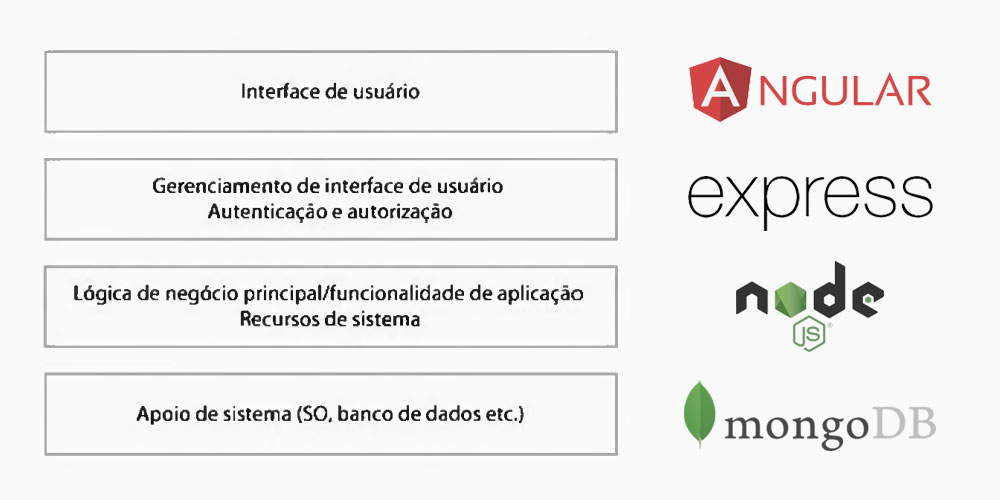
\includegraphics[scale=0.4]{mean-stack-flow}

\end{figure}

A Figura \ref{fig:MEANStackFlow} ilustra bem como a MEAN Stack segue o modelo de arquitetura em multicamadas apresentado no capítulo \ref{sec:Arquitetura}, apenas aplicando as tecnologias nas camadas exibidas na Figura \ref{fig:MultilayerArchitecture}.

Por utilizar quatro tecnologias distintas, podemos pensar que dará mais trabalho no desenvolvimento, mas ao contrário disso a MEAN Stack é utilizada até mesmo em curtas competições de programação conhecidas como \textit{Hackathon}, conseguindo protótipos de forma rápida e provando assim sua produtividade.

\subsection{MongoDB}

Um banco de dados flexível, poderoso, escalonável e de alta performance orientado a documentos. Lançado em 2009, escrito em C++, o MongoDB é gratuito e de código aberto.

Por ser orientado à documentos JSON, ou seja, retém os dados usando pares de chave/valor, podemos modelar dados de forma mais natural, utilizando a forma como os dados realmente serão utilizados em nossa aplicação, ao invés de criar várias ligações entre tabelas, o que o dá a característica ao MongoDB de banco não-relacional.

Para a execução de comandos no Mongo, existe um console que executa códigos JavaScript. Por esse motivo, desenvolvedores da linguagem terão facilidade em manter um banco MongoDB.

Com ele é possível receber a entrada no navegador com JavaScript, transportar a demanda para o \textit{back-end} ainda com a linguagem e, por fim, salvar um objeto no MongoDB ainda com o JavaScript. Naturalmente, o fluxo reverso também será tão prático quanto.

Em uma aplicação desenvolvida em cima do MEAN Stack o Mongo tem a responsabilidade de persistir os dados, ou seja, permite armazenar e recuperar dados. Ele representa na arquitetura multicamadas a camada de dados, como visto anteriormente no capítulo \ref{subsec:BancoDeDados}.

\subsubsection{Mongoose}

Com o Mongo é possível inserir qualquer formato JSON nas coleções, por esse motivo não há nenhum controle sobre os dados inseridos. Isso pode causar inconsistência nos dados, inserindo informações inválidas podendo quebrar a aplicação, deixando a responsabilidade para o desenvolvedor garantir a exatidão das informações.

Para resolver esse problema o Mongoose, que nos ajuda a modelar objetos de forma elegante para o MongoDB, ele fornece uma solução direta e baseada em esquemas para modelar os dados da nossa aplicação, incluindo conversão de tipo incorporada, validação, criação de consulta, ganchos de lógica de negócios e muito mais.

\subsection{Express}

Express é um \textit{framework} web rápido, flexível e minimalista para Node.js inspirado no Sinatra, um \textit{framework} para \textit{Ruby}. Ele facilita o desenvolvimento de aplicações web e \textit{APIs}, tanto pequenas quanto mais robustas, tornando fácil escalonar aplicações criadas com ele.

Com um conjunto de métodos utilitários \textit{HTTP} e \textit{middlewares} a seu dispor, criar uma \textit{API} robusta utilizando Express é rápido e fácil.

Na MEAN Stack, o Express tem a responsabilidade de disponibilizar \textit{endpoints} \textit{REST}, que serão consumidos pela aplicação cliente. Ele representa na arquitetura multicamadas a camada de controle, e também como camada de lógica de negócios como visto anteriormente nos Capítulos \ref{subsec:Servico} e \ref{subsec:Servidor}.

Através da Figura \ref{fig:MEANStackFlow} percebemos que o Express e Node.js fazem parte da mesma camada, o servidor.

Com o Express podemos criar nossa \textit{REST API}, configurando funções a serem executadas após o recebimento de chamadas em rotas, também conhecidas como URI's, pelos métodos \textit{HTTP} \textit{GET}, \textit{POST}, \textit{PUT}, \textit{PATH} e \textit{DELETE}.

\subsection{Angular}

Angular é um \textit{framework} JavaScript de código aberto, mantido pela Google. E tem como princípio "\textit{One framework. Mobile and Desktop}", que basicamente significa utilizarmos o Angular para criar nossa aplicação web e também aplicações para dispositivos móveis.

O \textit{framework} utiliza TypeScript como linguagem, isso pode nos ajudar a manter melhor um projeto grande, já que a tipagem de variáveis nos força a atribuir um valor ou objeto do tipo correspondente, dando assim de certa forma uma garantia de que não teremos problemas ao acessar algum dado. Mas no final todo o código é compilado e transformado em JavaScript.

A versão mais recente do Angular trabalha com componentes, que são trechos de códigos que definem elementos com aparência e comportamentos da interface. A ideia é que componentes sejam genéricos para que sejam utilizados e principalmente reutilizados em qualquer lugar da aplicação.

Na MEAN Stack, o Angular é responsável pela aplicação do usuário, ele cria interfaces dinâmicas sem manipulação direta no DOM, permite execução de lógica no \textit{client-side} além de facilitar a troca de dados \textit{REST}. Ele representa na arquitetura multicamadas a camada de apresentação, como visto anteriormente no Capítulo \ref{subsec:Cliente}.

Perceba que o Angular é apenas uma tecnologia que faz o papel de cliente na arquitetura, aqui poderíamos adotar qualquer outra ferramenta ou tecnologia, ou até mesmo diferentes tecnologias que consumissem o mesmo serviço, possibilitando assim criar infinitas aplicações clientes, como por exemplo um aplicativo para \textit{mobile} e outra aplicação mas voltada para web.

\subsection{Node.js}

O Node.js é uma plataforma de desenvolvimento construída sobre a linguagem JavaScript, por sua natureza assíncrona, executada pelo interpretador V8 criado pela Google e utilizado no Google Chrome, focado em migrar a linguagem JS para servidores. Foi criado pensando em um modelo não bloqueante para as operações de entrada e saída de dados (I/O - \textit{Input and Output}).

Neste modelo, as operações de I/O não bloqueiam o atendimento aos outros clientes, ou seja, quando são feitas operações como uma leitura no disco ou consulta de banco de dados, as requisições de outros clientes vão sendo enfileiradas. Após o processamento ser finalizado e respondido ao primeiro cliente, o próximo cliente é atendido.

Na MEAN Stack, o Node é o core pois ele é nosso ambiente de execução, que além de manter tudo disponível, contém as regras de negócio da nossa aplicação \textit{back-end}, também conhecida como \textit{server-side}. Ele representa na arquitetura multicamadas a camada de lógica de negócios, que trabalhando junto do Express também serve como camada de controle como visto anteriormente nos Capítulos \ref{subsec:Servidor} e \ref{subsec:Servico}.

\subsubsection{Node Package Manager}

O \textit{Node Package Manager}, mais conhecido como npm é o gerenciador de pacotes do Node.js. Com ele podemos fazer download de códigos, bibliotecas e \textit{frameworks} que nossos projetos podem usar, ou até mesmo ferramentas que exerçam alguma função em nosso sistema operacional.

O arquivo \verb|package.json| é responsável por gerenciar os pacotes cujo nosso projeto depende. Ele basicamente serve como uma lista para as dependências que nosso projeto necessita. Executando o comando do node \verb|npm install| automaticamente todas as dependências listadas serão baixadas.

Isso também nos ajuda a padronizar as versões de nossas dependências, facilitando informar os requisitos mínimos e atualizações, garantindo assim que todos os desenvolvedores terão a mesma versão em suas máquinas. Outra vantagem é para que outro desenvolvedor tenha acesso a nosso código, basta enviar o código em si, sem se preocupar com as dependências, pois basta ele executar o comando do node \verb|npm install| para fazer o download.

% -----------------------------------
% CHAPTER:
% Projeto
% -----------------------------------
\chapter{Projeto}

O projeto desenvolvido tem como objetivo abordar o assunto sobre informações ambientais e o desenvolvimento de uma aplicação que facilite o dia a dia de uma pessoa com o gerenciamento de irrigações de uma pequena plantação, ou apenas a grama de um jardim de forma sustentável.

A solução dos problemas ambientais tem sido considerada cada vez mais urgente para garantir o futuro da humanidade, e como hoje existem meios que facilitem o cuidado com o ambiente e a diminuição de desperdício, uma das formas de unirmos o cuidado com a diminuição de desperdício é desenvolvendo uma aplicação que tenha essa funcionalidade.

Para o desenvolvimento do projeto foi utilizado a linguagem JavaScript em conjunto dos \textit{frameworks} que compõem a MEAN Stack, seguindo a arquitetura apresentada no Capítulo \ref{sec:Arquitetura}.

Foi utilizado contêineres da tecnologia Docker para iniciar e gerenciar as camadas da aplicação. Um contêiner para cada responsábilidade, um para a Aplicação mobile, um para o Servidor e outro para o Banco de Dados, totalizando 3 contêineres. Sendo possível um maior controle por funcionalidade, podendo gerir e escalar em unidades, de forma que não influencie nos outros contêineres.

\begin{figure}[h]
	\centering

	\caption{Fluxo do projeto de aplicação criado} \label{fig:ProjectFlow}
    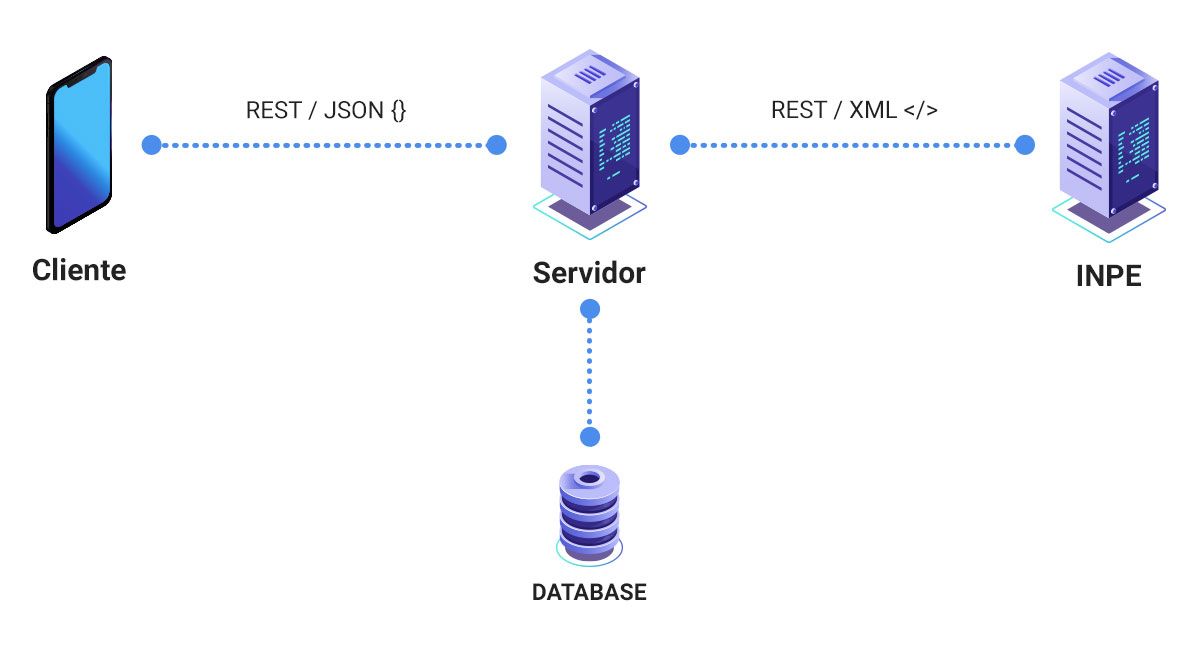
\includegraphics[scale=0.35]{project-flow} \\

\end{figure}

Conforme ilustrado na Figura \ref{fig:ProjectFlow}, o projeto tem o Cliente se comunicando com o Servidor que também realiza a comunicação com Banco de Dados e o serviço externo do INPE, sendo assim o fluxo das operações da aplicação.

\section{Aplicação mobile}

O aplicativo desenvolvido serve de gerenciador para o usuário cliente, onde ele pode se cadastrar como usuário, cadastrar e gerenciar os irrigadores além de saber a previsão do tempo para a cidade veículada para seu usuário e também para cada irrigador separadamente.

Seu papel é realizar a comunicação com o servidor através do protocolo \textit{REST}, enviando e pedindo dados, além de exibir as informações para o usuário.

Foi utilizado o \textit{Angular}, que é uma ferramenta presente na MEAN Stack, junto do \textit{Ionic}\footnote{\url{https://ionicframework.com/}}, que como descrito em seu própio site é um \textit{framework} que facilita a criação de aplicativos móveis e web progressivos de alto desempenho (ou PWAs) com aparência e beleza em qualquer plataforma ou dispositivo. Ele fornece componentes de interface do usuário, facilitando a criação de aplicativos com as linguagens HTML, CSS e JavaScript.

No build é possível escolher entre as plataformas \textit{iOS, Android, PWA} e até mesmo \textit{Desktop} para geração do arquivo final respectivo a plataforma escolhida.

\begin{figure}[h]
	\centering

	\caption{Aplicação cliente criada com \textit{Angular} para dispositivos móveis} \label{fig:ClientAppExample}
    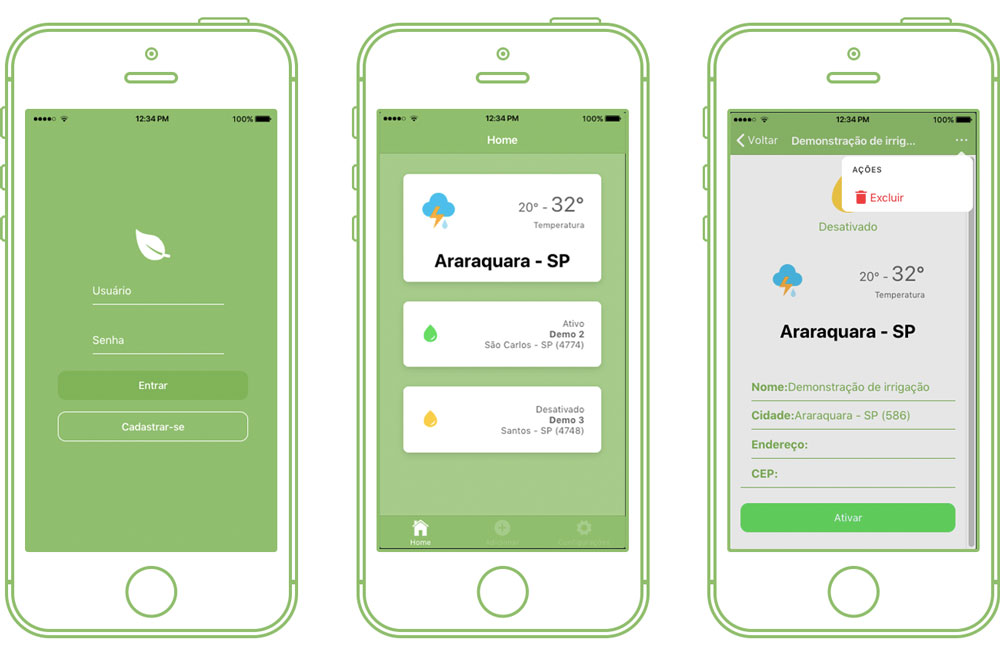
\includegraphics[scale=0.4]{client-app} \\

\end{figure}

A Figura \ref{fig:ClientAppExample} mostra a aplicação criada e algumas telas da aplicação com as quais o usuário pode interagir.

\section{Servidor}

\begin{figure}[h]
	\centering

    \caption{Serviço criado com \textit{Node.JS, Express} expõe a documentação e monitoramento em tempo real dos dados através do \textit{browser}} \label{fig:ServerAppExample}
    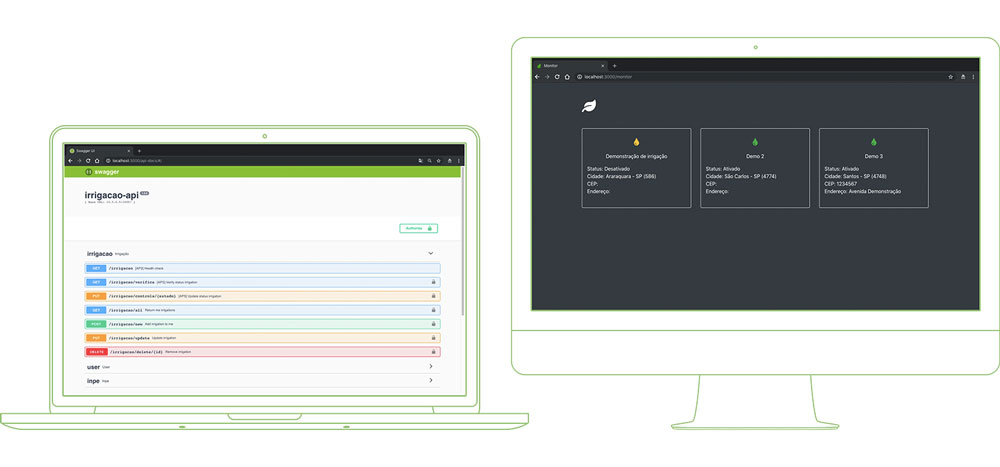
\includegraphics[scale=0.45]{server-app} \\

\end{figure}

\section{Banco de Dados}

% -----------------------------------
% CHAPTER:
% Conclusão
% -----------------------------------
\chapter{Conclusão}
Foi apresentado os benefícios na abordagem de utilizar apenas uma linguagem, no caso o JavaScript, em todas as camadas do desenvolvimento. Através da arquitetura multicamadas aplicamos a MEAN Stack, relacionando uma ferramenta para cada camada, mostrando ser capaz utilizar a linguagem nos mais diversos ambientes.

O JavaScript evolui a cada dia que passa, se eu pudesse apostar em uma linguagem pro futuro certamente escolheria o JS. Ao mesmo tempo que é uma linguagem de fácil aprendizado é uma linguagem forte e consolidada. Assim foi relatado a evolução da linguagem e sua  ampla utilização, para os mais diferentes tipos de sistemas, no contexto atual.

Também foi criado uma aplicação para mostrar na prática os conceitos aqui apresentados, e todo o código foi disponibilizado via GitHub, através do repositório\footnote{\url{https://github.com/rodrigocichetto/tcc}}, com todas as informações de licença e de como executar.

Desenvolver uma aplicação \textit{full stack} utilizando \textit{HTML, CSS} e \textit{JavaScript} proporcionou uma excelente experiência como desenvolvedor, pela flexibilidade de poder aplicar a lógica inteiramente com JavaScript, pelo rápido processamento, sobretudo no desenvolvimento da aplicação cliente, onde o aplicativo era renderizado no navegador web, bem mais rápido que o emulador \textit{Android} presente no \textit{Android Studio}, o que consequentemente exigiu menos processamento, além da vantagem de o \textit{build} ser multiplataforma, o que não acontece quando desenvolvemos no \textit{Android Studio}.

A aplicação desenvolvida teve também como objetivo abordar o assunto ambiental, visando facilitar o dia a dia de uma pessoa com os cuidados de uma plantação, ou apenas a grama de um jardim, de uma forma mais sustentável.

A solução dos problemas ambientais tem sido considerada cada vez mais urgente para garantir o futuro da humanidade, e como hoje temos meios que facilitem o cuidado com o meio ambiente e a diminuição de desperdício, uma das formas de unirmos o cuidado com a diminuição de desperdício é desenvolvendo uma aplicação que tenha tais funcionalidades.

% ----------------------------------------------------------
% ELEMENTOS PÓS-TEXTUAIS
% ----------------------------------------------------------
\postextual
% ----------------------------------------------------------

% ----------------------------------------------------------
% Referências bibliográficas
% ----------------------------------------------------------
% \bibliography{abntex2-modelo-references}
\bibliography{referencias-bibliograficas}

% ----------------------------------------------------------
% Glossário
% ----------------------------------------------------------
%
% Consulte o manual da classe abntex2 para orientações sobre o glossário.
%
%\glossary


% ----------------------------------------------------------
% Anexos
% ----------------------------------------------------------

% ---
% Inicia os anexos
% ---
\begin{anexosenv}

% % Imprime uma página indicando o início dos anexos
\partanexos

% -----------------------------------
% Primeiros passos Mongo
% -----------------------------------
\chapter{Primeiros passos Mongo}

Por padrão o terminal do Mongo inicia conectado ao banco de dados \verb|test|. Para mudarmos para outro banco de dados utilizamos o comando \verb|use nome_do_banco|. Caso o banco indicado não exista, o Mongo criará um novo assim que dados forem incluídos nele.

\textit{Insert}, através da função \verb|insert()| insere novos dados e pode receber como parâmetro um objeto JSON ou um array de objetos.

\begin{lstlisting}[language=javascript]
// Exemplo insert
db.nome_do_banco.insert()
\end{lstlisting}

\textit{Find}, através da função \verb|find()|, busca por objetos inseridos em uma \textit{collection}, podendo receber como parâmetro um objeto com os critérios de filtragem, ou nenhum para retornar todos os objetos.
 
\begin{lstlisting}[language=javascript]
// Exemplo find
db.nome_do_banco.find()
\end{lstlisting}

\textit{Update}, através da função \verb|update()| atualiza os dados, recebendo dois parâmetros, sendo o primeiro a condição para achar o documento, e o segundo o novo documento.

\begin{lstlisting}[language=javascript]
// Exemplo update
db.nome_do_banco.update()
\end{lstlisting}

\textit{Remove}, através da função \verb|remove()| remove os dados, podendo passar um parâmetro para informar qual objeto remover ou nenhum para remover todos, caso esse seja seu objetivo, também é possível utilizar o comando \verb|drop()|.

\begin{lstlisting}[language=javascript]
// Exemplo remove
db.nome_do_banco.remove()
// Exemplo drop
db.nome_do_banco.drop()
\end{lstlisting}

% -----------------------------------
% Primeiros passos Express
% -----------------------------------
\chapter {Primeiros passos Express}

Para criarmos um servidor com o Express, necessitamos primeiro do Node.js e o NPM instalados, caso não saiba como instalá-los veja a explicação no Anexo \ref{anexo:NodePrimeirosPassos}.

No terminal inicie um projeto node a partir do comando \verb|npm init|, preencha as informações e então execute o comando \verb|npm install express| dentro do diretório do seu projeto para instalar o express. Desta maneira conseguimos importar o express para nosso código. Finalmente é só criar um arquivo \verb|app.js| com o código abaixo.

\begin{lstlisting}[language=javascript]
const express = require('express');
const app = express();
const PORT = 3000;

app.get('/', (req, res) => {
   res.send('Hello World');
});

app.listen(PORT, () => {
    console.log('Servidor disponivel na porta ' + PORT);
});
\end{lstlisting}

Para iniciar o servidor basta executar o comando \verb|node app.js|, enfim abra seu navegador no endereço \href{http://localhost:3000}{http://localhost:3000} ele deve retornar nosso \textit{Hello World}.

\section{Express Generator}

Com apenas o comando \verb|express nome_da_app| do Express Generator ele já estrutura uma aplicação Express simples. Após a execução do comando ele irá criar um novo diretório com o nome da aplicação informado anteriormente, contendo arquivos e dependências necessárias. 

Antes de iniciarmos o servidor Express devemos instalar as dependências através do comando \verb|npm install| que irá baixar as dependências de acordo com o arquivo \verb|package.json| gerado anteriormente. Enfim é hora de iniciar a aplicação executando o comando \verb|npm start| e acessá-la pelo endereço \href{http://localhost:3000}{http://localhost:3000}.

\begin{figure}[h]
	\centering

	\caption{Aplicação gerada pelo Express Generator} \label{fig:ExpressGeneratorApp}
    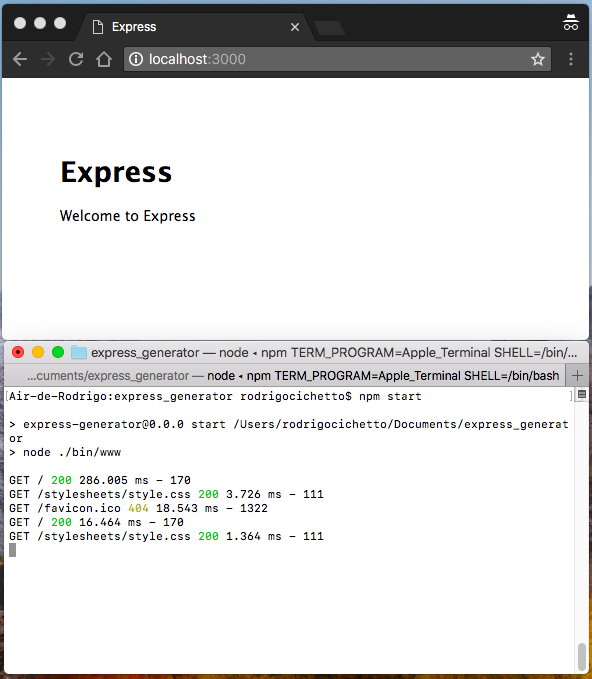
\includegraphics[scale=0.5]{express-generator-app} \\

\end{figure}

Essa página só é exibida porque no arquivo \verb|routes/index.js| está configurado a rota padrão para que renderize o arquivo \verb|views/index.jade| passando o título com o valor Express, sendo interpretado pela \textit{template engine} JADE, configurada por padrão pelo Express Generator.

Para saber mais opções de geração de estruturas através do Express Generator, execute o comando \verb|express -h|.

% -----------------------------------
% Primeiros passos Angular CLI
% -----------------------------------
\chapter{Primeiros passos Angular CLI} 

Instalado a partir do comando do node \verb|npm install -g @angular/cli|, o Angular CLI é uma interface de linha de comando para o Angular, que nos permite trabalhar de forma mais amistosa com a tecnologia.

Com o Angular CLI é possível criar projetos e estruturá-los a partir do comando \verb|ng|. Por exemplo, para criar um novo projeto, basta executar o comando \verb|ng new app-name|, assim não precisamos nos preocupar com a estrutura inicial do projeto e suas dependências cruciais para o funcionamento do Angular. 

Para iniciar o servidor com o Angular, basta executar o comando \verb|ng serve| e abrir seu navegador no endereço \href{http://localhost:4200}{http://localhost:4200}.

Ainda é possível criar componentes, pipes, módulos, diretivas e serviços de forma rápida com o comando \verb|ng generate|.

% \pagebreak
\begin{figure}[h]
	\centering

	\caption{Aplicação gerada pelo Angular Cli} \label{fig:AngularCliApp}
    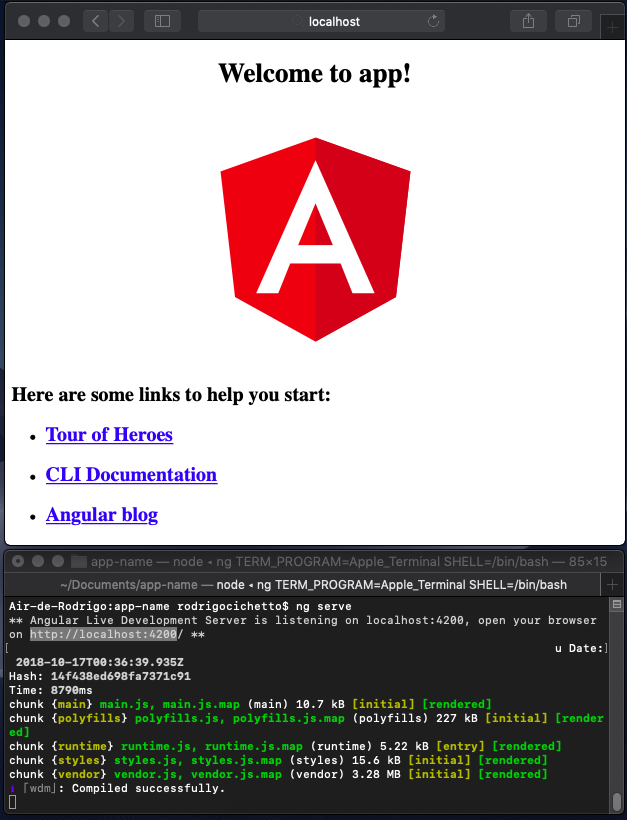
\includegraphics[scale=0.4]{angular-cli-app} \\

\end{figure}

% -----------------------------------
% Primeiros passos Node.js
% -----------------------------------
\chapter {Primeiros passos Node.js}
\label{anexo:NodePrimeirosPassos}

Instalar o Node.js é muito simples, basta acessar o link \href{https://nodejs.org/en/download/}{https://nodejs.org/en/download/} e baixar o instalador ou seguir as instruções de instalação de acordo com o seu sistema operacional.

Para iniciar um projeto em Node.js devemos primeiro criar um diretório, em seguida acessá-lo via terminal, enfim digitamos o comando \verb|npm init| e preenchemos as informações de acordo com nosso projeto. Perceba que ele gerou o arquivo \verb|package.json| com as informações preenchidas no comando via terminal.

Agora é só começar a desenvolver e instalar suas dependências, que devem ficar salvas no arquivo gerado anteriormente.

% \pagebreak
\begin{figure}[h]
	\centering

  \caption{Exemplo de configurações preenchidas no comando npm init} \label{fig:NpmInitExample}
    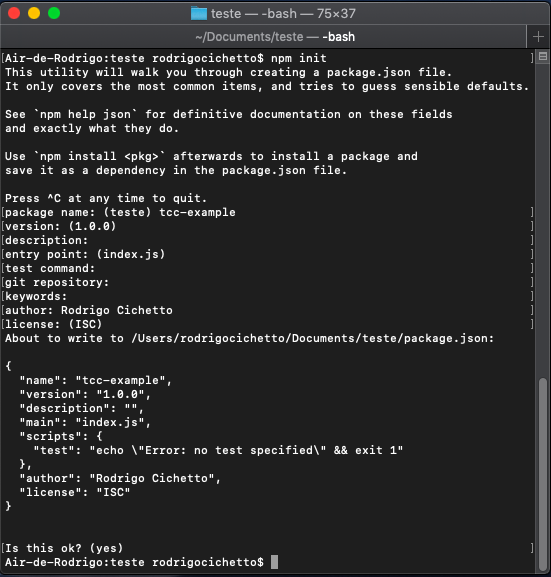
\includegraphics[scale=0.5]{npm-init-example} \\

\end{figure}

% % ---
% \chapter{Morbi ultrices rutrum lorem.}
% % ---
% \lipsum[30]

% % ---
% \chapter{Cras non urna sed feugiat cum sociis natoque penatibus et magnis dis
% parturient montes nascetur ridiculus mus}
% % ---

% \lipsum[31]

% % ---
% \chapter{Fusce facilisis lacinia dui}
% % ---

% \lipsum[32]

\end{anexosenv}

%---------------------------------------------------------------------
% INDICE REMISSIVO
%---------------------------------------------------------------------
%\phantompart
\printindex
%---------------------------------------------------------------------

\end{document}